\documentclass[a4paper,10pt]{article}
\usepackage[utf8]{inputenc}
\usepackage[margin=1in]{geometry}
\usepackage{graphicx}
\usepackage{listings}

\begin{document}

\begin{titlepage}
\begin{center}
\vspace*{1cm}

\huge{\textbf{Reversi using Minimax and Aplha-Beta Pruning}}

\vspace{0.5cm}
CS621 Project

\vspace{1.5cm}

\Large{\textbf{Anshul Gupta (16305R001) \\ Himanshu Agarwal (163050001)}}

\vfill

\vspace{0.8cm}


\includegraphics[scale=0.05]{IITB.png}
\end{center}
\end{titlepage}
 
\section*{High Level Structure}
The code is divided into 3 files: \texttt{client.py}, \texttt{board.py} and \texttt{ai.py}.

\subsection*{client.py}
\texttt{client.py} is responsible for establishing the connection with the server and interacting with it. It has two modes: \textit{Human v/s Computer} and \textit{Computer v/s Computer}.\\[0.2cm]
If the former is chosen, it gives a prompt for entering the desired moves. If the latter is chosen, it asks for an \textit{Intelligence Level} which can take values from $1 - 4$ (4 being the highest).\\[0.2cm]
It automatically terminates the game if the board becomes full or both server and client runs out of moves.

\subsection*{board.py}
\texttt{board.py} manages all the operations on the board. These include \textit{printing the board}, \textit{updating the board}, \textit{finding the legal moves} and \textit{validating the moves}.\\[0.2cm]
This file cannot be executed directly but imported in \texttt{client.py} and \texttt{ai.py} to perform board operations on the objects of this class.

\subsection*{ai.py}
\texttt{ai.py} handles all the intelligent operations. AI class takes input as the current state of the board and enumerates all possible moves for the player and opponent for the specified level (default = 4).\\[0.2cm]
It then evaluates the situation of the game and finds the best possible move for the player using a heuristic function. It optimizes the searching using \textit{Aplha-Beta Pruning}.\\[0.2cm]
This file also cannot be executed directly but imported in \texttt{client.py} to generate the tree and get the best move.

\begin{figure*}[h]
\vspace{1cm}
\centering
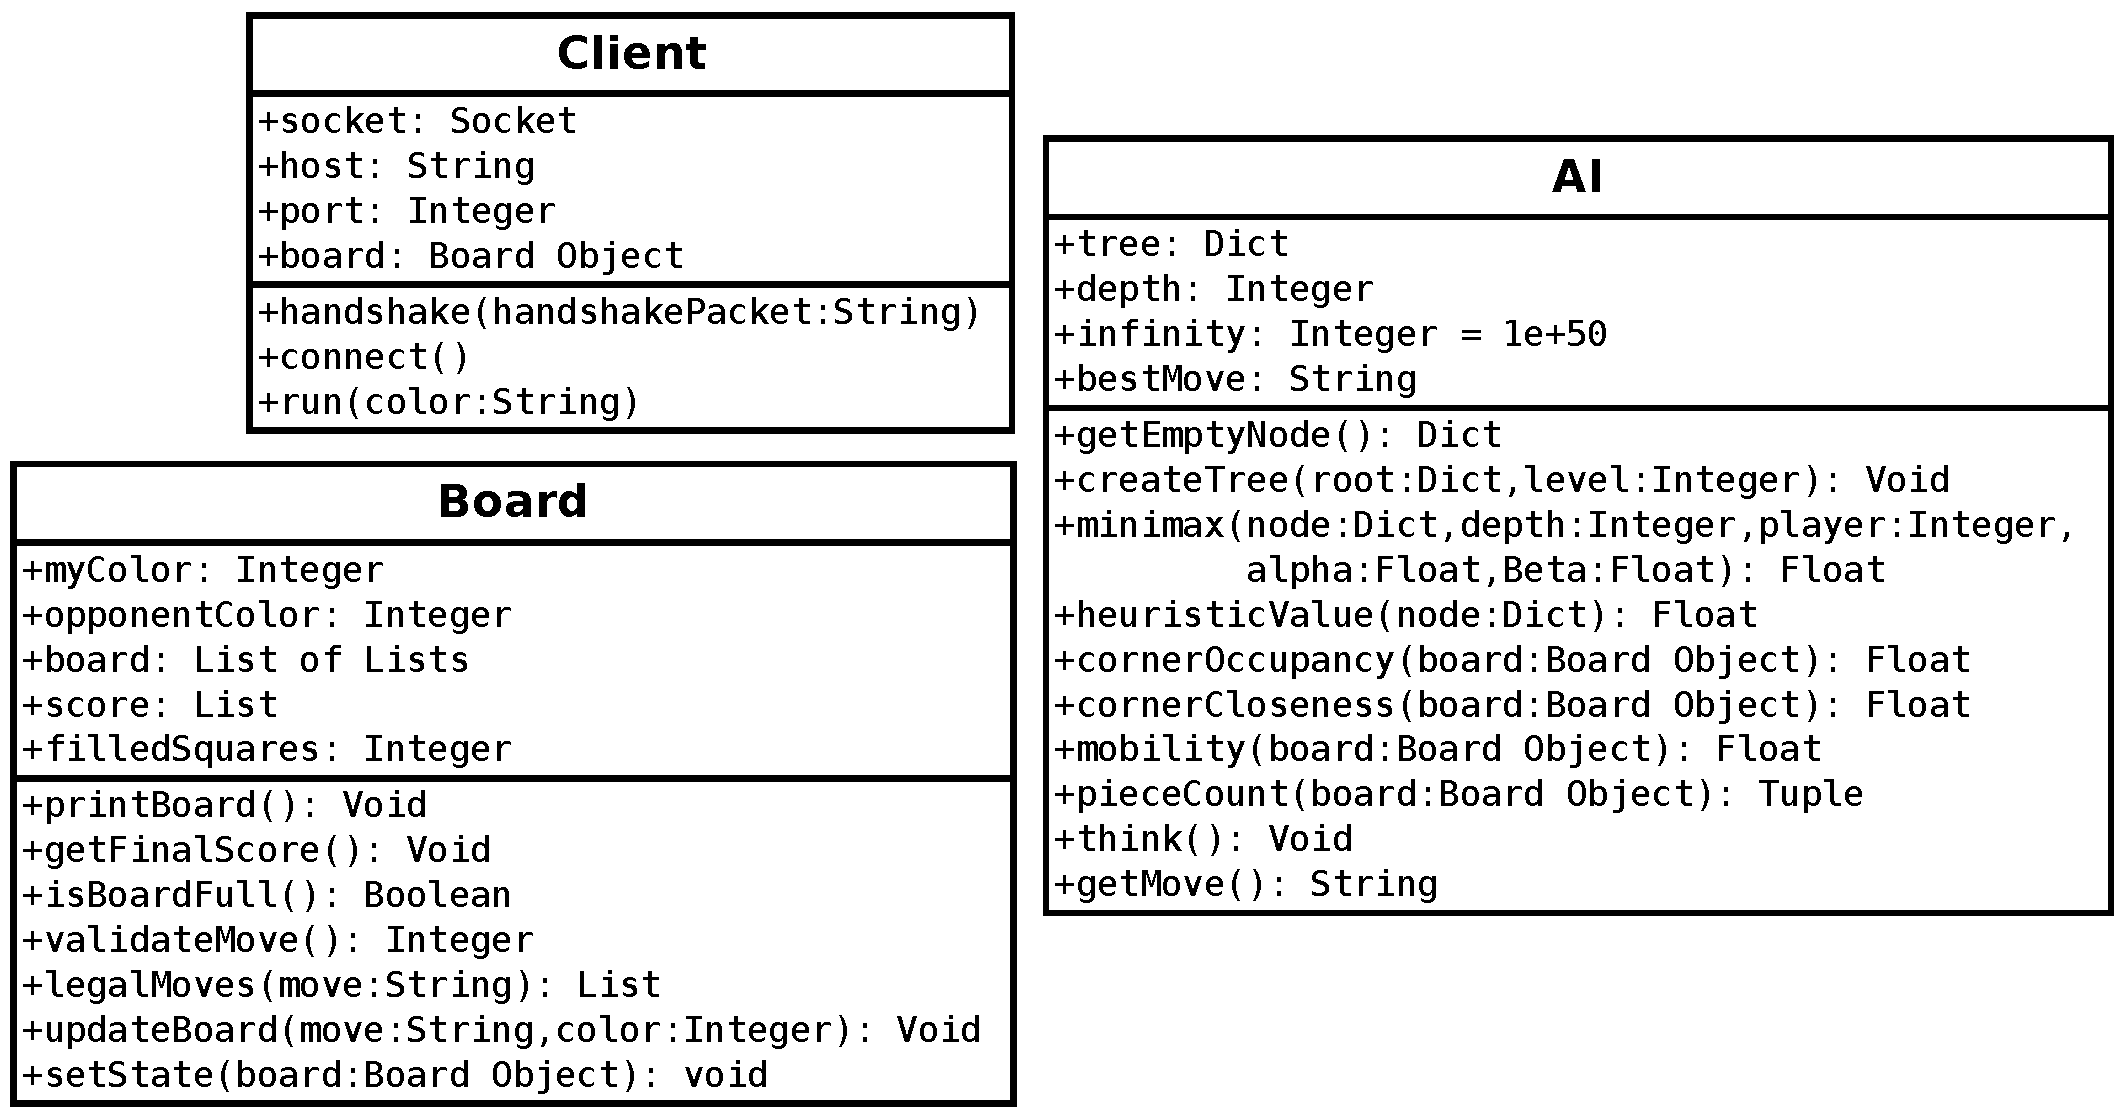
\includegraphics[scale=0.42]{Classes.pdf}
\end{figure*}

\newpage
\section*{Heuristic Used}
Heuristic is calculated based on six factors some of which are static and some are dynamic.
\subsubsection*{pieceValue}
It is calculated by counting the pieces of both players. If a player has more pieces than other, it has more advantage.
\begin{verbatim}
if myPieces > opponentPieces:
  pieceValue = (100 * myPieces) / (myPieces + opponentPieces)
elif myPieces < opponentPieces:
  pieceValue = (-100 * opponentPieces) / (myPieces + opponentPieces)
\end{verbatim}

\subsubsection*{diskSquares}
It is a static factor. Each square of the board has a integer value (+ve or -ve). If a player's piece is on a square, the value of that square is added to it's points, if opponent's piece is on a square, the value of that square is subtracted from the points.

\subsubsection*{frontierValue}
Frontier pieces are those which are on the perimeter (having alteast one empty neighbor). This is a negative factor.
\begin{verbatim}
if myFtrPieces > opponentFtrPieces:
  FrontierValue = (-100 * myFtrPieces) / (myFtrPieces + opponentFtrPieces)
elif myFtrPieces < opponentFtrPieces:
  FrontierValue = (100 * opponentFtrPieces) / (myFtrPieces + opponentFtrPieces)
\end{verbatim}

\subsubsection*{cornerValue}
Corner piece has an advantage that if it is occupied, it can never be flanked. So if a player has pieces on corners, they will have a positive effect on the player.
\begin{verbatim}
cornerValue = 25 * (myCornerPieces - opponentCornerPieces)
\end{verbatim}

\subsubsection*{cornerClosenessValue}
The pieces which are the immediate neighbors of the corner, they have a disadvantage that they can be flanked easily and the opponent will gain a corner position. This is a negative factor.
\begin{verbatim}
cornerClosenessValue = -12.5 * (myPieces - opponentPieces)
\end{verbatim}

\subsubsection*{mobilityValue}
Mobility is the number of moves a player has. More the number of moves, more advantage a player will have.
\begin{verbatim}
if myMoves > opponentMoves:
  return (100 * myMoves) / (myMoves + opponentMoves)
elif myMoves < opponentMoves:
  return (-100 * opponentMoves) / (myMoves + opponentMoves)
\end{verbatim}

\subsubsection*{Heuristic Value}
The final heuristic value is calculated using:
\begin{verbatim}
heuristicValue = (10 * diskSquares)
		  + (10 * pieceValue)
		  + (74.396 * frontierValue)
		  + (801.724 * cornerValue)
		  + (382.026 * cornerClosenessValue)
		  + (78.922 * mobilityValue)
\end{verbatim}
\newpage

\end{document}
